%!TEX program = xelatex
%!TEX options=--shell-escape

\documentclass{beamer}

\setbeamerfont{title}{series=\bfseries}
\setbeamerfont{frametitle}{series=\bfseries}

\definecolor{OxfordBlue}{RGB}{0,33,71}
\setbeamercolor{title}{fg=OxfordBlue}
\setbeamercolor{frametitle}{fg=OxfordBlue}
\setbeamercolor{section in toc}{fg=black}
\setbeamercolor{description item}{fg=black}
\setbeamertemplate{description item}{\bfseries\insertdescriptionitem}
\setbeamertemplate{itemize item}{\color{OxfordBlue}$\blacktriangleright$}
\setbeamerfont{block title}{series=\bfseries}
\setbeamercolor{block title}{use={frametitle},fg=frametitle.fg,bg=frametitle.bg}

\AtBeginSection[]{
  \begin{frame}
    \vfill\centering\usebeamerfont{title}\insertsectionhead\par\vfill
  \end{frame}
}

\newcommand{\hl}[1]{\textcolor{OxfordBlue}{\textbf{#1}}}

\usepackage{fontspec}
\setmonofont[Scale=MatchUppercase]{Fira Mono}
\setsansfont{FoundrySterling}[
  UprightFont=*-Book,
  BoldFont=*-Bold,
  ItalicFont=*-BookItalic
]

\usetheme{default}
\beamertemplatenavigationsymbolsempty

\usepackage{graphicx}
\usepackage{pgffor}
\usepackage{hyperref}
\usepackage{booktabs, colortbl}

\usepackage[cache=false]{minted}
\usemintedstyle{tango}

\title{\huge Another way to use a map\LARGE\\at the School of Geography}
\date{\scriptsize January 24\textsuperscript{th} 2019}
\author{Nicolas Payette}
\institute{%
  
\includegraphics[height=1cm]{images/geog-brand-pos}%
  
\includegraphics[height=1cm]{images/ox_brand_cmyk_pos.eps}
}

\begin{document}

\maketitle

\begin{frame}{Overview}\LARGE
\tableofcontents
\end{frame}

\section{A word about functions}

\begin{frame}
  \begin{figure}
    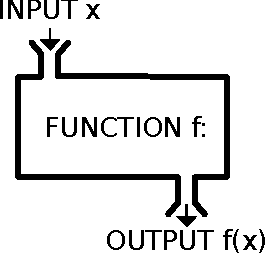
\includegraphics[height=0.8\textheight]{images/function}
  \end{figure}
  \vfill\hfill\tiny%
  \textcolor{gray}{\url{https://en.wikipedia.org/wiki/Function_(mathematics)}}%
\end{frame}

\begin{frame}\LARGE
  \vfill
  A \hl{higher-order function}:\vskip 2mm
  \begin{itemize}\Large
    \item takes one or more functions as inputs
    \item and/or outputs a function.
  \end{itemize}
  \vfill\pause
  \hl{\texttt{map}} is a higher-order function that:\vskip 2mm
  \begin{itemize}\large
    \item takes a function and a collection of things as inputs
    \item and outputs another collection of things.
  \end{itemize}
  \vfill
\end{frame}

\section{Mapping over a collection}

\foreach \i in {0,...,13} {%
  \begin{frame}{}
    \includegraphics[width=\textwidth]{images/map-\i.png}%
    \vfill\hfill\tiny%
    \textcolor{gray}{\url{https://en.wikipedia.org/wiki/Map_(higher-order_function)}}%
  \end{frame}%
}

\begin{frame}[fragile]{Python}
  \inputminted{python}{../demo-map.py}
\end{frame}
\begin{frame}[fragile]{Julia}
  \inputminted[fontsize=\small]{julia}{../demo-map.jl}
\end{frame}
\begin{frame}[fragile]{R}
  \inputminted{R}{../demo-map.R}
\end{frame}
\begin{frame}[fragile]{NetLogo}
  \inputminted[fontsize=\footnotesize,style=NetLogo]{nlogo}{../demo-map.nls}
\end{frame}

\begin{frame}{NetLogo}
  \begin{table}\Huge
    \newcommand{\arr}{\Large\textcolor{gray}{$\longleftrightarrow$}}
    \begin{tabular}{@{}rcl@{}}
      \arrayrulecolor{gray}
      \toprule
      \hl{Agentsets} &      & \hl{Lists}       \\
      \midrule
      \texttt{of}    & \arr & \texttt{map}     \\
      \texttt{with}  & \arr & \texttt{filter}  \\
      \texttt{ask}   & \arr & \texttt{foreach} \\
      \bottomrule
    \end{tabular}
  \end{table}
\end{frame}

\begin{frame}[fragile]{Java}
  \inputminted[fontsize=\footnotesize]{java}{../demo-map.java}
\end{frame}
\begin{frame}[fragile]{Scala}
  \inputminted{scala}{../demo-map.scala}
\end{frame}

\section{A tiny practical example}

\begin{frame}[fragile]{Read all CSV files in a folder}
  \Large
  \textcolor{gray}{\textbf{R:}}\par
  \inputminted[fontsize=\scriptsize]{R}{../read-csv.R}
  \vskip 5mm
  \textcolor{gray}{\textbf{Julia:}}\par
  \inputminted[fontsize=\scriptsize]{Julia}{../read-csv.jl}
\end{frame}

\section{Mapping over two collections}

\begin{frame}[fragile]{Python}
  \inputminted{python}{../demo-map2.py}
\end{frame}
\begin{frame}[fragile]{Julia}
  \inputminted[fontsize=\small]{julia}{../demo-map2.jl}
\end{frame}
\begin{frame}[fragile]{R}
  \inputminted[fontsize=\small]{R}{../demo-map2.R}
\end{frame}
\begin{frame}[fragile]{NetLogo}
  \inputminted[fontsize=\small,style=NetLogo]{nlogo}{../demo-map2.nls}
\end{frame}
\begin{frame}[fragile]{Java}
  \inputminted[fontsize=\scriptsize]{java}{../demo-map2.java}
\end{frame}
\begin{frame}[fragile]{Scala}
  \inputminted{scala}{../demo-map2.scala}
\end{frame}

{\setbeamercolor{background canvas}{bg=black}
\begin{frame}[plain]
  \makebox[\linewidth]{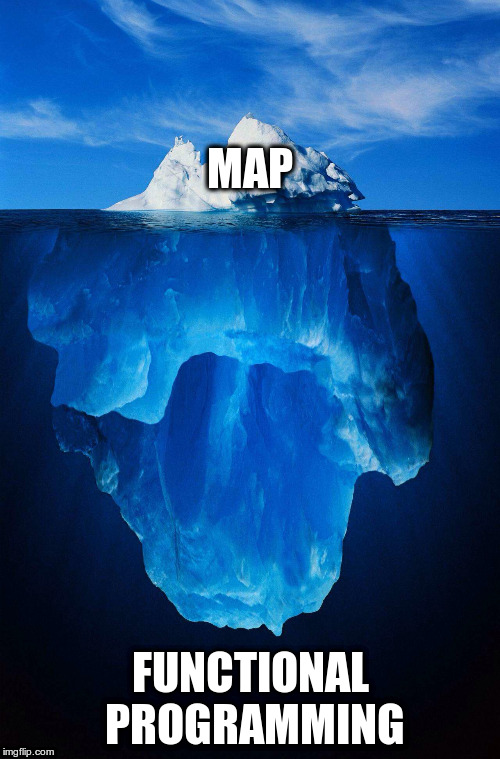
\includegraphics[height=\paperheight]{images/iceberg}}
\end{frame}}

\begin{frame}
  \begin{center}
    \hl{\huge Code and slides:}\par\vskip1cm
    \url{https://github.com/nicolaspayette/demo-map}
  \end{center}
\end{frame}
\end{document}
